\graphicspath{{./ch_carbon_dephasing_purified/figures/}}


\chapter{Storing a quantum state during optical excitation of a quantum network node}
\label{ch:CDP}

\begin{center} 
    \vspace{-1cm} {M.S.~Blok, K. ~van Bemmelen, N.~Kalb, A.~Reiserer, T.H.~Taminiau and R.~Hanson} 
\end{center}

\vspace{0.5cm} 

The ability to locally store a quantum state in a quantum network node while establishing entanglement with a distant node is a crucial prerequisite for implementing entanglement distillation, purification and quantum repeater protocols\cite{Bennett_Phys.Rev.Lett._1996,Campbell_Phys.Rev.Lett._2008,Briegel_Phys.Rev.Lett._1998,Childress_Phys.Rev.Lett._2006}. For quantum network nodes based on NV centers in diamond, nearby $^{13}$C-spins are a prime candidate for such a quantum memory. The challenge is that these nuclear spins have a constant coupling to the optically active electron spin, resulting in possible dephasing of the stored state when the electron is reset multiple times as required for generating remote entanglement. In chapter \ref{ch:CDL} we discussed an analytical model to describe this process and found that nodes with low electron-nuclear coupling strength and fast electron reset are expected to provide the best performance. Here we present preliminary experimental results to test our model in an isotopically purified sample where $^{13}$C-spins with coupling strengths of < 1 kHz can be located and controlled. We find that multiple resets of the electron spin indeed induce dephasing of the nuclear-spin quantum memory and that this process can be suppressed by reducing the electron reset time. While the data qualitatively agrees with our model, the observed decoherence rate is faster than predicted indicating that we are limited by an additional dephasing process. Nonetheless our results show that a $^{13}$C-spin allows for the storage of a quantum state during 200 repetitions with very little loss of fidelity ($99 \%$ fidelity with initial state).
\clearpage

\section{Introduction}

 \begin{figure*}
	\centering
	\includegraphics[width=130mm]{Fig1}
	\caption{\label{fig:cdp-fig1} \textbf{} (a)Dynamical Decoupling spectroscopy of the $^{13}$C-spin bath. Grey lines are the expected collapses of the signal due to interaction with the $^{13}$C-spin bath. (b) Two $^{13}$C-Spins can be identified, red (green) line is a simulation of the resulting signal for the interaction with a single spin with hyperfine constants of $A_{par} = ...$ and $A_{perp}$ ($A_{par} = ...$ and $A_{perp}$) (c) Free induction decay of a single carbon spin with and without repetitive reset }
\end{figure*}

 \begin{figure*}
	\centering
	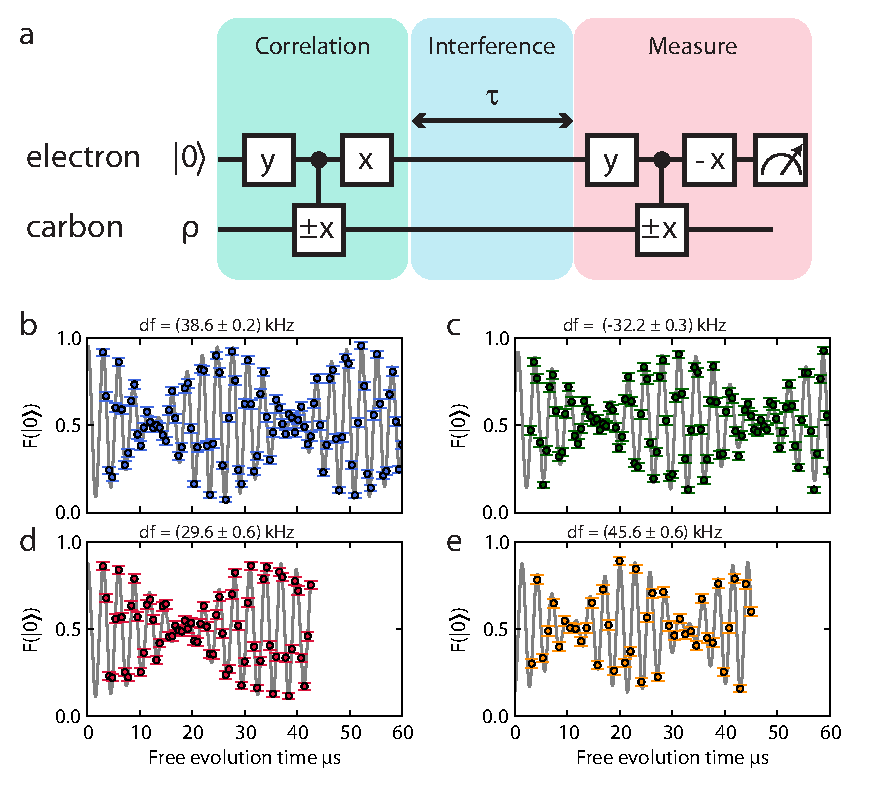
\includegraphics[width=130mm]{Fig2}
	\caption{\label{fig:cdp-fig2} \textbf{Reset of the electron spin} (a) Measurement of the timescale of the reset process. Plotted is the probability of preparing $m_s = 0$ after preparing $m_s = \pm 1$ as a function of repump time and power (b) Fitted time constant of the reset process as a function of reset power.}
\end{figure*}

 \begin{figure*}
	\centering
	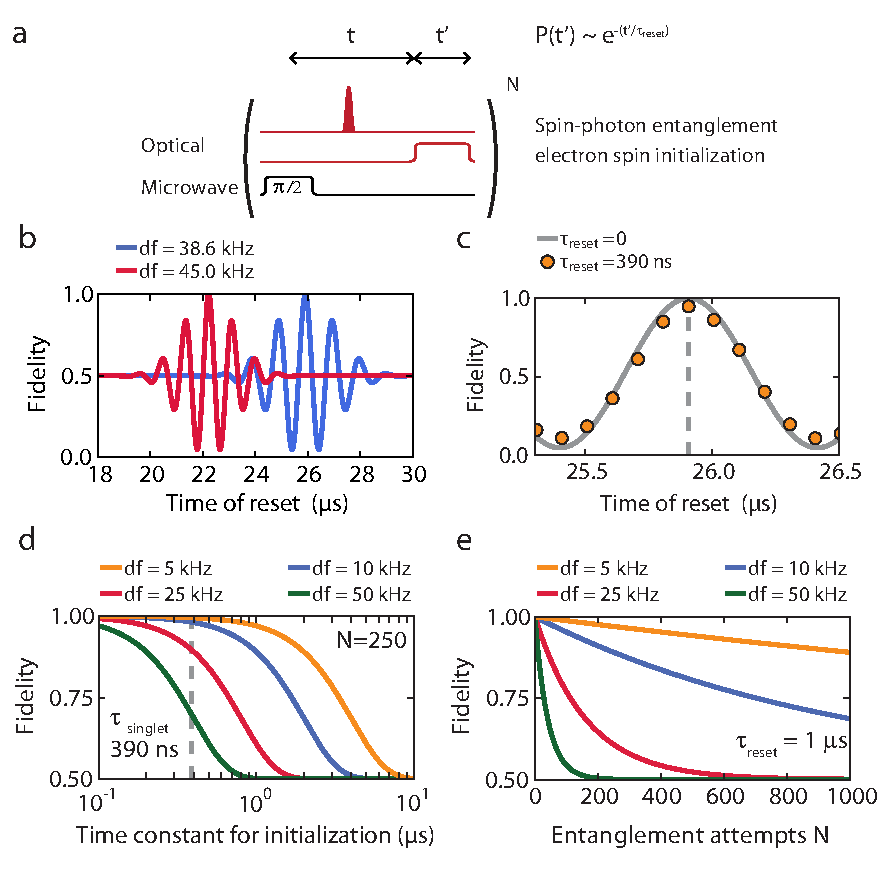
\includegraphics[width=130mm]{Fig3}
	\caption{\label{fig:cdp-fig3} \textbf{} (a) Result of tomography (measuring X,Y and Z) for varying number of resets. (b) }
\end{figure*}
\newpage
\bibliographystyle{../thesis}
\bibliography{cdp}


